%-------------------------------------------------------------
% Language
% Use the option "language=EN" to set the beamer theme in English. Use
% the option "language=ES" to set the beamer theme in Spanish.

% Colors
% Use the option "color=white" to set the background in white and the
% bottom bar in blue. Use the option "color=blue" to set the
% background in blue and the bottom bar in white. Use the option
% "color=blue2" to set the background in blue and the bottom bar in
% blue.

% Font Color
% Use the option "fontc=black" to set the font color in black. If this
% argument is not given the default color is set depending of the
% color scheme selected.

% Notes:
% Do not use \large inside multicols
% Enumerate require \justifying command
% Tables captions bellow the tabular
% With citations, note = {} may only work for @misc

% Credits: https://github.com/alejogm0520 & Samuel Plazas Escudero
%-------------------------------------------------------------

%--Principal packages
\documentclass[xcolor=table, aspectratio=43,8pt, notheorems]{beamer} % 4:3; can be 16:9; [...,8pt,t] in order to start text of all frames on the upper part; add: draft to not compile figures.
\usetheme[language=EN, color=white]{EAFIT}
\usepackage[english]{babel}
\usepackage[utf8]{inputenc}
\usepackage[T1]{fontenc}
\usepackage{algorithm2e}
\usepackage{amsmath,amsfonts,amssymb,cancel}
\newcommand{\overbar}[1]{\mkern 1.5mu\overline{\mkern-0.5mu#1\mkern-0.5mu}\mkern 1.5mu}

% Equations; physics is optional and sometimes problematic!
\usepackage{verbatim} % Environments, \begin{comment}
\usepackage{fancyvrb}
%--Arial
\usepackage{helvet}\renewcommand{\familydefault}{\sfdefault}
% It's ok
%--David Plazas recommended
%\usepackage{libertine} % Normal
%--Carlos Cuartas 
%\usepackage[T1]{fontenc}\usepackage{lmodern} % Best
%--Beamer packages
\usepackage{tikz} % For making vectorized figures, arrows
\usepackage{ifthen} % For specifying conditionals for sections
\usepackage{ragged2e}\justifying % Whole text justified, except enumerate: add \justifying
\usepackage{multicol} % Multiple columns in one frame
%--Tables-Figures
\usepackage{natbib}
\usepackage{url}
\usepackage{booktabs,multirow} % Bookstyle tables
\usepackage{array} % Custom width and centered
\newcolumntype{P}[1]{>{\centering\arraybackslash}p{#1}} % horizontal centering but use custom width
\newcolumntype{M}[1]{>{\centering\arraybackslash}m{#1}} % horizontal and vertical centering but use custom width
%-Figure label
\usepackage[labelsep=period,justification=justified,format=plain]{caption} % Dot instead of colon and justified caption
%--Figure
\usepackage{graphicx,subcaption} % Figures and subfigures
\usepackage{media9} % video and audio
%-Figure-Table on top
\usepackage{float} % Allows to put H instead of ht
\setbeamertemplate{caption}[numbered] % Numbered captions
%---------TOC
\setbeamertemplate{section in toc}[sections numbered]
\setbeamertemplate{subsection in toc}[subsections numbered]
\setbeamerfont{section in toc}{size=\small}
\setbeamerfont{subsection in toc}{size=\footnotesize}
\setbeamertemplate{subsection in toc}{\leavevmode\leftskip=3.2em\rlap{\hskip-2em\inserttocsectionnumber.\inserttocsubsectionnumber}\inserttocsubsection\par} % Indented subsection
\setcounter{tocdepth}{2} % Toc depth, put 1 for only showing there the sections and 2 to include sections
%---------Cite
\usepackage{bibentry} % Full cite foot
\nobibliography* % Full cite foot
\setbeamertemplate{bibliography item}[triangle]% [online][book][article][triangle][text]; Or: \setbeamertemplate{bibliography item}{\insertbiblabel} 
\usepackage{etoolbox} % Package for using justified bibliography 
\apptocmd{\thebibliography}{\justifying}{}{} % Justified bibliography 
%---------Footnotes
\setbeamercolor{footnote}{fg=white} % Footnote white 
\setbeamercolor{footnote mark}{fg=.} % Takes the color depending on the circumpstance
\setbeamercolor{bibliography entry author}{fg=white} % Allows to have white footnote bibs
\setbeamertemplate{footnote}
{
  \hspace*{-1cm} % Horizontal movement
  \vspace*{-3.12cm} % Vertical movement
  \parbox[c][3.64cm]{10.6cm}{\tiny\noindent\insertfootnotemark\insertfootnotetext} % b: bottom, height: 3.3cm, horizontal length: 10.6cm (max horizontal)
% If there are problems, put \vspace*{-2.87cm} and \parbox[c][3.3cm]
% or \vspace*{-2.88cm} and \parbox[c][3.4cm]
% or \vspace*{-3.05cm} and \parbox[c][3.6cm]
% or \vspace*{-3.12cm} and \parbox[c][3.64cm]
}
\renewcommand{\footnoterule}{\kern -3pt \hrule width \textwidth height 0pt\kern 3pt} % No footnoterule
\usepackage{perpage}\MakePerPage{footnote} % Footnote numbered per frame
\renewcommand{\thefootnote}{\Roman{footnote}} % Roman number in footnote
                                              % Cutom: \fnsymbol{footnote}
%------------------------------------
%---------Numbered Slides and Sections
\setbox0=\hbox{\subsecname\unskip}\ifdim\wd0=0pt\else%
 ~--~\insertsubsectionhead
\fi
%------Numbering section: title in bold, centered and with a line
\newcommand{\numb} 
{
  \setbeamertemplate{frametitle}
  {
    \ifx\insertsubsection\empty % No subsection
         \bfseries\thesection.~\insertframetitle~\color{black}\par\vskip-5pt\hrulefill % \centering
    \else % subsection
         \bfseries\thesection.~\insertframetitle~\color{black}\par\vskip-9pt\hrulefill\par\vskip3pt{\large\thesection.\thesubsection~\insertframesubtitle} % Subsection with smaller size;
    \fi
  }
}
%------No numbering section: title in bold, centered and with a line
\newcommand{\nonumb}
{
  \setbeamertemplate{frametitle}{\bfseries\color{black}\centering\insertframetitle\par\vskip-6pt\hrulefill}
}
%------------------------------------
%--No hyphenation on text
\tolerance=1
\emergencystretch=\maxdimen
\hyphenpenalty=10000
\hbadness=10000
%------------------------
%---------Itemize justified in beamer
\makeatletter
\renewcommand{\itemize}[1][]{
  \beamer@ifempty{#1}{}{\def\beamer@defaultospec{#1}}
  \ifnum \@itemdepth >2\relax\@toodeep\else
    \advance\@itemdepth\@ne
    \beamer@computepref\@itemdepth % Sets \beameritemnestingprefix
    \usebeamerfont{itemize/enumerate \beameritemnestingprefix body}
    \usebeamercolor[fg]{itemize/enumerate \beameritemnestingprefix body}
    \usebeamertemplate{itemize/enumerate \beameritemnestingprefix body begin}
    \list
      {\usebeamertemplate{itemize \beameritemnestingprefix item}}
      {\def\makelabel##1{
          {
            \hss\llap{{
                \usebeamerfont*{itemize \beameritemnestingprefix item}
                \usebeamercolor[fg]{itemize \beameritemnestingprefix item}##1}}
          }
        }
      }
  \fi
  \beamer@cramped
  \justifying % Justified itemize
  \beamer@firstlineitemizeunskip
}
\makeatother
%------------------------
%---------get current section name for showing it at its begining
\usepackage{nameref}
\makeatletter
\newcommand*{\currentname}{\@currentlabelname}
\makeatother
%---------Shows in which section we are at the begining of each one
\begin{comment}
\AtBeginSection[]
{
\begin{frame}[plain,noframenumbering]
  \begin{beamercolorbox}[ht=\paperheight,wd=\paperwidth, center]{Portada}
    \begin{center}\textbf{\LARGE \currentname}\end{center} % Leave the next space mandatorily

    \vspace{0.44\paperheight}
  \end{beamercolorbox}
\end{frame}
}
\end{comment}

\usepackage[absolute,overlay,showboxes]{textpos}
%\usepackage[texcoord,grid,gridunit=mm,gridcolor=red!10,subgridcolor=green!10]{eso-pic} % Helping grids, comment when publishing
%---------NOTES IN BEAMER
\AtBeginNote{\Huge}\newcommand{\notei}[1]{\note[item]{\Huge{\textcolor{blue}{#1}}}} % Use \notei{text} everywhere % [1] means one parameter located in #1 (input). 
\setbeamertemplate{note page}[plain] % Plain style for notes page
\setbeameroption{show notes} % {show notes} or {hide notes}
% \setbeameroption{show notes on second screen=right}
% as well you can use \documentclass[notes=only] at the beginning of the code
%-----------More elaborated notes
%\setbeamercolor{note page}{bg=white!90!black, fg=black}
%\setbeamercolor{note title}{bg=white!30!red, fg=black}
%\setbeamercolor{note date}{parent=note title}
%---------Itemize, enumberate and lists inside them
%\setbeamertemplate{itemize/enumerate body begin}{\LARGE} % Body
\setbeamertemplate{itemize/enumerate subbody begin}{\Large} % Subbody
%---------COLOR DEFINITIONS
\definecolor{azure(colorwheel)}{rgb}{0.0, 0.5, 1.0} % Define colors here
\definecolor{blue(ryb)}{rgb}{0.01, 0.28, 1.0}

\usepackage[normalem]{ulem}
\useunder{\uline}{\ul}{}


\usepackage{mathtools}
 \usepackage{tikz}
\DeclarePairedDelimiter{\ceil}{\lceil}{\rceil}
%%%%%%%%%%%%%%%%%%%%%%%
%Start of the Document%
%%%%%%%%%%%%%%%%%%%%%%%

%---------COVER PAGE
\title{$\pmb{2^k}$ FACTORIAL DESIGN}
\author{\normalfont\texorpdfstring{Presented by:\\ David Plazas E.\\Mateo Restrepo S.\\Juan Sebastian Cárdenas-Rodríguez.}{}}

\def\eafit{Universidad EAFIT}
\def\materia{Modelation and Simulation V}
\def\fecha{2019} % or put the exact date
% to add more def, search for "Dirección" in beamerthemeEAFIT.sty

%\includeonly{Slides/0_cover_title,ex_beamer,Slides/refs_thanks}
\usepackage{amsthm}
 % to number
\setbeamertemplate{theorems}[numbered]
 % insert bellow all blocks you want in italic
\newtheorem{theorem}{Theorem}[section] % to number according to section
\theoremstyle{definition} % insert bellow all blocks you want in normal text
\newtheorem{definition}{Definition}[section] % to number according to section
\newtheorem*{idea}{Proof idea} % no numbered block
\newtheorem{example}{Example}[section]
\newtheorem{corollary}{Corollary}[theorem]

\theoremstyle{plain}
\begin{document}

\nonumb % Not numbered titles
\begin{frame}
% Portada Inspira Crea Transforma
\end{frame}
%%%%%%%%%%%%%%%%%%%%%%%%%%%%%%%%%%%%%%%%%%%%%%%%%%%%%%%%%%%%%%%%%%%%%%%%%%%%
\begin{frame}
\begin{center}
  \titlepage % Cover page
\end{center}
\end{frame}
%%%%%%%%%%%%%%%%%%%%%%%%%%%%%%%%%%%%%%%%%%%%%%%%%%%%%%%%%%%%%%%%%%%%%%%%%%%%
\begin{frame}{CONTENIDO}
\begin{multicols}{2}
  \tableofcontents
\end{multicols}
\end{frame}
\numb % Numbered titles
%\begin{comment}
\section{Factorial Design $2^2$}
\subsection{Theory}
\begin{frame}{Factorial Design $\pmb{2^2}$}
\framesubtitle{Problem Definition}

\begin{multicols}{2}
\textbf{Problem}
\begin{itemize}
    \item Two factors with two possible levels. \pause
    \item Simulation model.\pause
    \item It's desired to change a result of the simulation.
\end{itemize}

\columnbreak
\pause
\textbf{Objective}\\ \vspace{0.1cm} Analyze the effect that the factors have in the output of the model.
\end{multicols}
\pause
\begin{multicols}{2}
\textbf{Notation}
\begin{itemize}
    \item $n \rightarrow$ number of runs per treatment.
    \item $y_{i\lambda} \rightarrow$ output of $i^{\text{th}}$ simulation for the $\lambda^{\text{th}}$ treatment. 
    \item For each treatment $\lambda := \sum_{i=1}^n y_{i\lambda}$
\end{itemize}

\columnbreak
\centering
\textbf{Yates notation}
\begin{table}[]
\centering
\begin{tabular}{ccc}
\hline
      & Factor $A$ & Factor $B$ \\ \hline
$(1)$ & Low        & Low        \\
$a$   & High       & Low        \\
$b$   & Low        & High       \\
$ab$  & High       & High       \\ \hline
\end{tabular}
\label{tab:yates}
\end{table}
\end{multicols}
\end{frame}

\begin{frame}{Factorial Design $\pmb{2^2}$}
\framesubtitle{Workflow}
\begin{multicols}{2}
\onslide<2->{\textbf{Contrasts}\\
\begin{table}[H]
\centering
\begin{tabular}{lccc}
\hline
      & \multicolumn{1}{l}{Cont $A$} & \multicolumn{1}{l}{Cont $B$} & \multicolumn{1}{l}{Cont $AB$} \\ \hline
$(1)$ & -                                & -                                & +                                 \\
$a$   & +                                & -                                & -                                 \\
$b$   & -                                & +                                & -                                 \\
$ab$  & +                                & +                                & +                                 \\ \hline
\end{tabular}
\label{tab:contrast}
\end{table}}
\onslide<3->{
Equations:
$$\begin{array}{l}{\text { Cont } A=[a+a b-b-(1)]} \\ {\text { Cont } B=[b+a b-a-(1)]} \\ {\text { Cont } A B=[a b+(1)-a-b]}\end{array}$$
}
\onslide<4->{
\textbf{Effects}
\begin{equation*}
    \text{Effect } \chi = \dfrac{\text{Cont } \chi}{2n}, \quad \chi = A, B, AB
\end{equation*}}
\columnbreak
\onslide<1->{
\begin{figure}
    \centering
    \only<1>{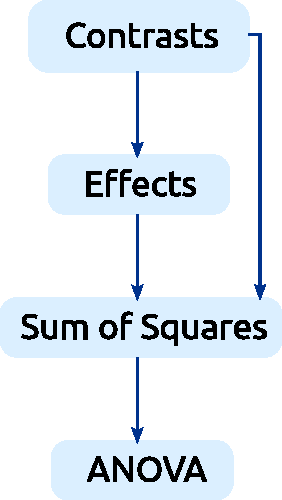
\includegraphics[scale=0.6]{images/proc.pdf}}
    \only<2>{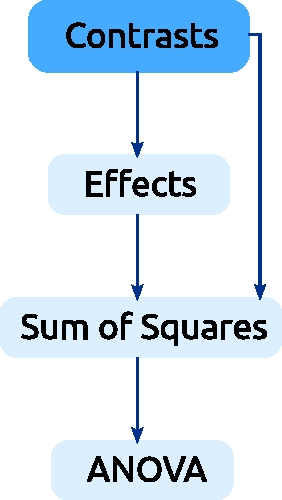
\includegraphics[scale=0.6]{images/contrast.pdf}}
    \only<3>{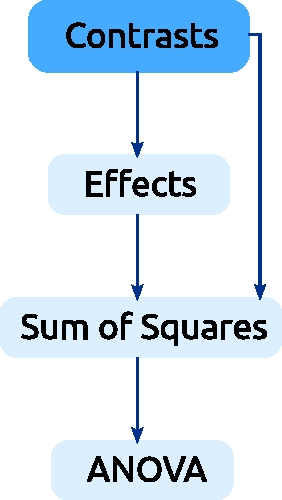
\includegraphics[scale=0.6]{images/contrast.pdf}}
    \only<4>{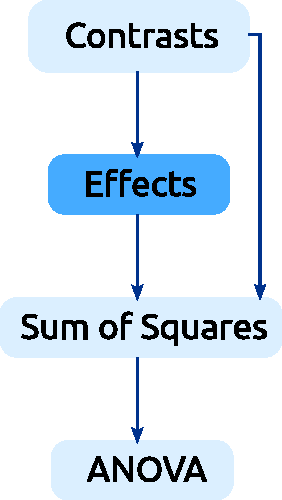
\includegraphics[scale=0.6]{images/effects.pdf}}
\end{figure}}
\end{multicols}
\end{frame}

\begin{frame}{Factorial Design $\pmb{2^2}$}
\framesubtitle{Workflow}
\begin{multicols}{2}
\onslide<1->{
\textbf{Squared sum}
\begin{equation*}
    \begin{split}
    \text{SS}_{\chi} =& \dfrac{(\text{Cont }\chi)^2}{2^2n},  \quad \text{df}_\chi = 1\\
    \text{SS}_t =& \sum_\lambda \sum_{i=1}^n y_{i\lambda}^2 -
    \dfrac{y_{..}^2}{2^2n},\quad \text{df}_t=2^2n-1\\
    \text{SS}_e =& \text{SS}_t - \sum_\chi \text{SS}_\chi, \quad \text{df}_e = 2^2(n-1)
    \end{split}
\end{equation*}
\onslide<2->{ 
\textbf{Average Squares:}
\begin{equation*}
    \text{AS}_\beta=\dfrac{\text{SS}_\beta}{df_\beta}
\end{equation*}}
}
\columnbreak
\onslide<1->{
\begin{figure}
    \centering
    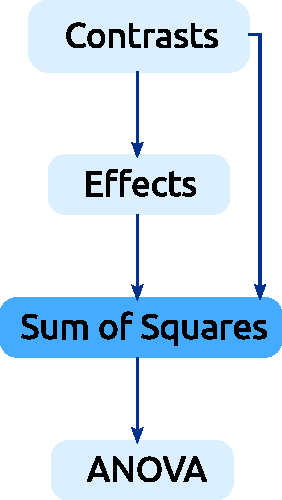
\includegraphics[scale=0.6]{images/sum.pdf}
\end{figure}}
\end{multicols}
\end{frame}


\begin{frame}{Factorial Design $\pmb{2^2}$}
\framesubtitle{Workflow}\begin{multicols}{2}
\textbf{ANOVA:}\\\vspace{0.5cm} 
$H_0:$ Effect A $ =0$\\ \vspace{0.3cm}
$H_0:$ Effect B $   =0$\\\vspace{0.3cm} 
$H_0:$ Effect AB $ =0$\\\vspace{0.5cm} 

Test:
\begin{align*}
    F_{0\chi} &= \dfrac{\text{AS}_{\chi}}{\text{AS}_e}, \quad F \sim \mathbb{F}_{(1,2^2(n-1))}\\ \vspace{0.5cm}
    P_{0\chi} &= \mathrm{P}(F>F_{0\chi})\\\vspace{0.5cm}
\end{align*}
Given a significance level $\alpha$, the null hypothesis ($H_0$) is rejected if $P_{0\chi} < \alpha$
\columnbreak
\begin{figure}
    \centering
    \centerline{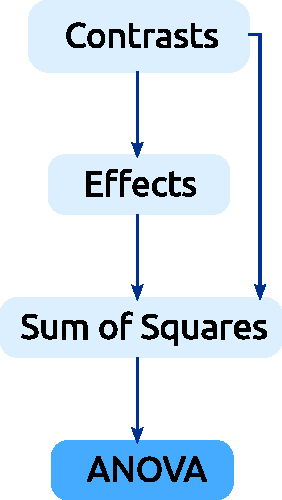
\includegraphics[scale=0.6]{images/anoa.pdf}}
\end{figure}
\end{multicols} 
\end{frame}

\subsection{Example}
\begin{frame}{Factorial Design $\pmb{2^2}$}
\framesubtitle{Example}
    Joe’s parlour is open from 9.00am to 7.00pm and he and his fitters work throughout that period if there is work to be done. Motorists arrive and wait for Joe to inspect their car’s exhaust system.Joe drives the car onto any free hydraulic ramp for inspection.Joe then advises the customer on the necessary work and customers elect to stay or go off elsewhere. When the fitter is finished, Joe inspects the work and, if satisfactory, he prints out the bill for the driver, who then pays and leaves. If Joe decides that the work is not satisfactory  then the fitter must rework the job – and this may take as long as the original work. 
    
    Joe would like some advice from you. He needs to know how many fitters and ramps he should employ in the parlour (currently, three ramps and two fitters) \citep{pidd1998computer}.
\end{frame}
\section{Factorial Design $\pmb{2^k}$}
\subsection{Yates Notation}
\begin{frame}{Factorial Design $\pmb{2^k}$}
\framesubtitle{Yates Notation}
    This notation can be extended for any value of $k$.
\begin{table}[H]
\begin{tabular}{lccc}
\hline
      & Factor $A$ & Factor $B$ & Factor $C$ \\ \hline
$(1)$ & Low        & Low        & Low        \\
$a$   & High       & Low        & Low        \\
$b$   & Low        & High       & Low        \\
$c$   & Low        & Low        & High       \\
$ab$  & High       & High       & Low        \\
$ac$  & High       & Low        & High       \\
$bc$  & Low        & High       & High       \\
$abc$ & High       & High       & High       \\ \hline
\end{tabular}
\end{table}
    Normally we are interested in treatment with a singular or double factor.
\end{frame}

\subsection{The Best ANOVA}
\begin{frame}{Factorial Design $\pmb{2^k}$}
    \framesubtitle{The Best ANOVA}
It's necessary to make first ANOVA to select which factors don't have a significant impact.\\ \pause

Let $\chi^*$ be the selected factors and $k^*$ the number of selected factor. Then, the \textbf{best ANOVA} test is made:

\begin{align*}
    T_{0\chi^*} &= \dfrac{\text{Effect } \chi^*}{\sqrt{\dfrac{\text{AS}_e}{n2^{k^*-2}}}}, \quad T \sim t_{(\alpha,2^{k^*}(n-1))}\\ \vspace{0.5cm}
    P_{0\chi^*} &= \mathrm{P}(T>T_{0\chi^*})\\\vspace{0.5cm}
\end{align*}
The null hypothesis ($H_0$) is rejected if $P_{0\chi^*} < \alpha$

\end{frame}

\begin{frame}{Factorial Design $\pmb{2^k}$}
\framesubtitle{Non-Replicated $\pmb{2^k}$ Factorial Design}
\begin{itemize}
    \item For $k\geq5$, the experimentation can be unmanageable (e.g. $2\times2^5=64$ runs).
    \item Only one replica is desirable for $k\geq4$.
    \item Make fractions of the complete experiments, analyze them separately and decide if it is necessary to continue the experimentation.
    \item Take samples to estimate the error and apply an approximated ANOVA procedure.
\end{itemize}
\begin{table}[]
\centering
\begin{tabular}{ccc}
\hline
\textbf{Design} & \textbf{Replicas}                        & \textbf{Runs} \\ \hline
$2^2$           & 3 or 4                                   & 12, 16        \\
$2^3$           & 2                                        & 16            \\
$2^4$           & 1 or 2                                   & 16, 32        \\
$2^5$           & fraction $2^{5-1}$ or 1                  & 16, 32        \\
$2^6$           & fraction $2^{6-2}$ or fraction $2^{6-1}$ & 16, 32        \\
$2^7$           & fraction $2^{7-3}$ or fraction $2^{7-2}$ & 16, 32        \\ \hline
\end{tabular}
\end{table}
\end{frame}

%\section{Conclusiones}
%\begin{frame}{Conclusiones}
%    \begin{itemize}
%    \item 
%\end{itemize}
%\end{frame}
\nonumb % Not numbered titles
%\addcontentsline{toc}{section}{\small\protect\numberline{}{REFERENCIAS BIBLIOGRÁFICAS}} % Separated from other contents, for small number of contents
\addcontentsline{toc}{section}{\small REFERENCES} % Closer from other contents, for large number of contents
\nocite{*} % All citations showed (take care with fraud!)
%%%%%%%%%%%%%%%%%%%%%%%%%%%%%%%%%%%%%%%%%%%%%%%%%%%%%%%%%%%%%%%%%%%%%%%%%%%%
\section*{REFERENCES}
\begin{frame}[allowframebreaks]{REFERENCES} %  and put before {REFEREN...}
\begingroup % Group for changing the color
\renewcommand{\color}[1]{} % Allows to have black bibs and white footnote bibs
\small{\bibliographystyle{IEEEtran}} % Size of text; acm or gatech-thesis or ieeetr or ieeetran or icontec or iso690
\bibliography{ref}
\endgroup % Group for changing the color
% pdflatex -> bibtex -> pdflatex -> pdflatex
\end{frame}
%%%%%%%%%%%%%%%%%%%%%%%%%%%%%%%%%%%%%%%%%%%%%%%%%%%%%%%%%%%%%%%%%%%%%%%%%%%%
% Thank-slide
\begin{frame}[plain,noframenumbering] % No frame number
	\begin{beamercolorbox}[ht=\paperheight,wd=\paperwidth, center]{Portada}
		\begin{center}\Huge\textbf{Thank you}\end{center} % Or Thanks; leave the next space mandatorily
		
		\vspace{0.44\paperheight}
    \end{beamercolorbox}
\end{frame}
%%%%%%%%%%%%%%%%%%%%%%%%%%%%%%%%%%%%%%%%%%%%%%%%%%%%%%%%%%%%%%%%%%%%%%%%%%%%


\end{document}